\chapter{Introduzione al Deep Learning}

Ciò che bisogna consolidare prima di immergerci nello studio del Deep Learning è la differenza fra Machine Learning e Deep Learning. Per far questo bisogna analizzare quello che si fa con i programmi di Machine Learning, riferiamoci a uno specifico caso d'uso. Partiamo considerando il riconoscimento di un'immagine. Nel Machine Learning si parte dal creare un programma, il quale deve essere in grado, data un'immagine, di estrarre alcuni attributi per poi utilizzarli all'interno di un modello di ML e riconoscere immagini della stessa tipologia. Il passo ulteriore che viene effettuato nel Deep Learning è a monte, ossia durante la selezione degli attributi, quì noi costruiamo una gerarchia degli stessi, avendo la possibilità di stabilire attributi di basso, medio e alto livello. Questa selezione avviene con la combinazione di modelli di Machine Learning, creando nella sua complessità un meccanismo automatico più raffinato e profondo, da cui nasce il Deep Learning.

\begin{figure}
    \centering
    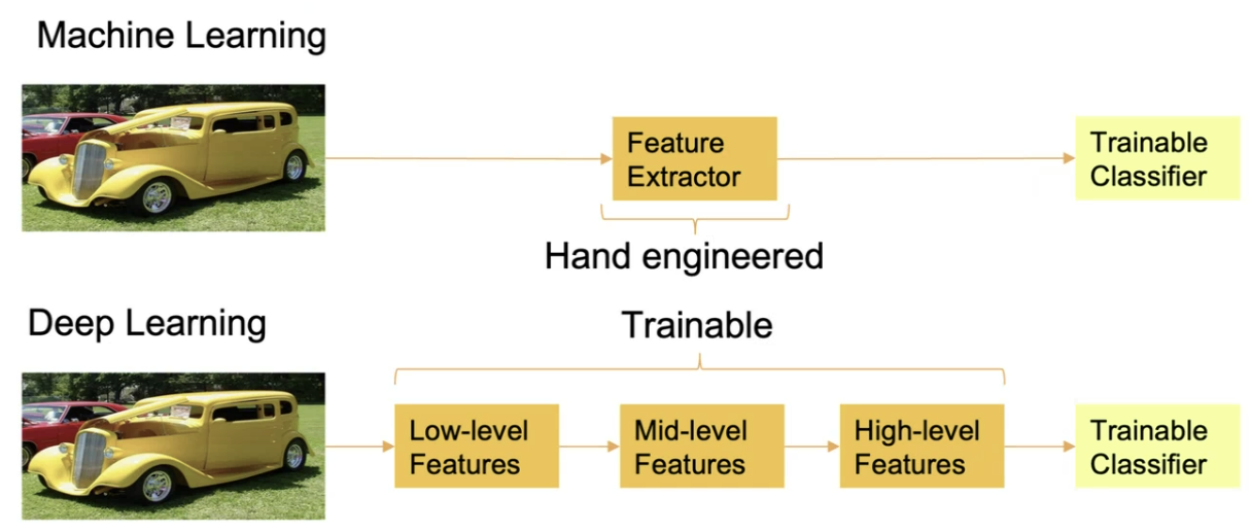
\includegraphics[width=0.75\linewidth]{figure/DeepMachineDiff.png}
    \caption{Schema rappresentativo della principale differenza fra un modello di Machine Learning e di Deep Learning}
    \label{fig:DLMLDiff}
\end{figure}

\section{Definizione}
Il Deep Learning dunque è una sotto-disciplina del Machine Learning la quale utilizza reti neurali profonde, ossia delle reti neurali con numerosi hidden-layer, per poter estrarre delle rappresentazioni gerarchiche dai dati. A differenza dei metodi tradizionali di Machine Learning, i quali richiedono l'ingegnerizzazione manuale delle caratteristiche, il Deep Learning è in grado di apprendere automaticamente rappresentazioni multi-livello, direttamente dai dati grezzi. Questo approccio, si è dimostrato particolarmente efficace in campi come la visione artificiale, il riconoscimento vocale e l'elaborazione del linguaggio naturale.

\section{Esempio: Il dataset MNIST}
MNIST è un dataset ampiamente utilizzato per il riconoscimento di cifre scritte a mano. Composto da 60.000 immagini di addestramento e 10.000 immagini di test, ognuna delle quali è una griglia $28\times28$ di pixel in scala di grigi. L'obiettivo di un modello di apprendimento automatico addestrato su MNIST, risulta essere quello di classificare correttamente ogni immagine in una delle 10 categorie (da 0 a 9). Questo dataset viene spesso utilizzato come benchmark, per poter valutare le prestazioni di nuovi algoritmi di apprendimento profondo.
\\
\begin{figure}[ht]
    \centering
    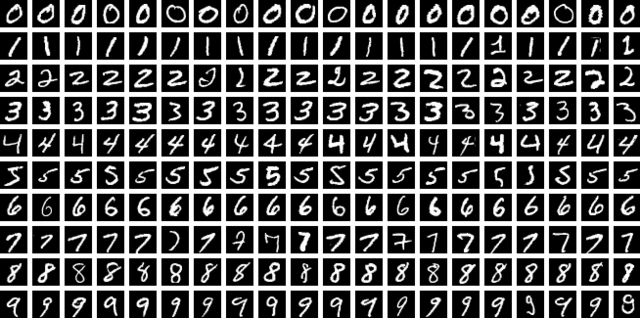
\includegraphics[width=0.75\textwidth]{figure/MNIST_dataset_example.png}
    \caption{Un estratto delle immagini presenti all'interno del dataset del MNIST.}
\end{figure}

\section{Grafi Computazionali}
Un Grafo computazionale rappresenta il flusso di operazioni effettuate tra variabili, viene utilizzato per modellare i calcoli svolti da una rete neurale. Ogni nodo del grafo rappresenta un'operazione matematica, mentre i bordi o archi, rappresentano i flussi di dati. Utilizzando questa struttura, possiamo visualizzare il flusso delle informazioni e il processo di apprendimento della rete. Ad esempio, in una rete neurale profonda, ogni livello applica una trasformazione, tramite l'utilizzo di una funzione di attivazione generando un output, il quale verrà poi propagato fino al livello finale, per ottenerne una previsione. Il modello utilizzato da noi, distingue nettamente i vari elementi tramite l'utilizzo di forme e colori, in modo da essere maggiormente intuitivo, avendo una differenza fra input, funzioni deterministiche e funzioni scalari (Figura~\ref{fig:parModel}).

\begin{figure}
    \centering
    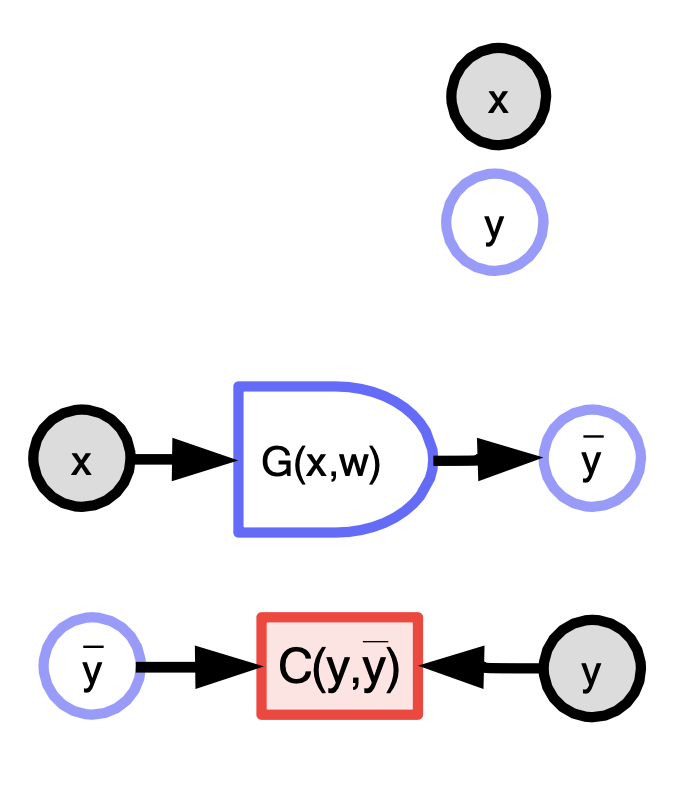
\includegraphics[width=0.40\linewidth]{figure/ParametriModel.png}
    \caption{Notazione dei nostri modelli, dall'alto verso il basso ci sono: Variabili, Funzione deterministica e Funzione scalare}
    \label{fig:parModel}
\end{figure}

\section{Funzione di costo}
Una \textbf{Funzione di Costo} è un'operazione riportabile tramite l'utilizzo dei nostri grafi computazionali (Figura~\ref{fig:costFunction}). Questa funzione misura l'errore pesente tra l'output fornito dal modello, dunque una predizione e l'output desiderato, essa, risulta essere fondamentale per il processo di apprendimento. Il modello, cerca di minimizzare questa funzione di costo, in inglese Loss Function (per questo si parla spesso di perdita), aggiustando i pesi della rete di volta in volta attraverso un algoritmo di ottimizzazione. Una delle funzioni di costo più comuni è la Mean Squared Error (MSE), definita come:
\begin{equation}
    C(y, \hat{y}) = \frac{1}{n} \sum_{i=1}^{n} (y_i - \hat{y}_i)^2
\end{equation}
Dove $y_i$ rappresenta il valore reale e $\hat{y}_i$ l'output predetto dal modello per il campione $i$-esimo. Minore è il valore della funzione di costo, migliore sarà la capacità del modello di effettuare previsioni accurate.

\begin{figure}
    \centering
    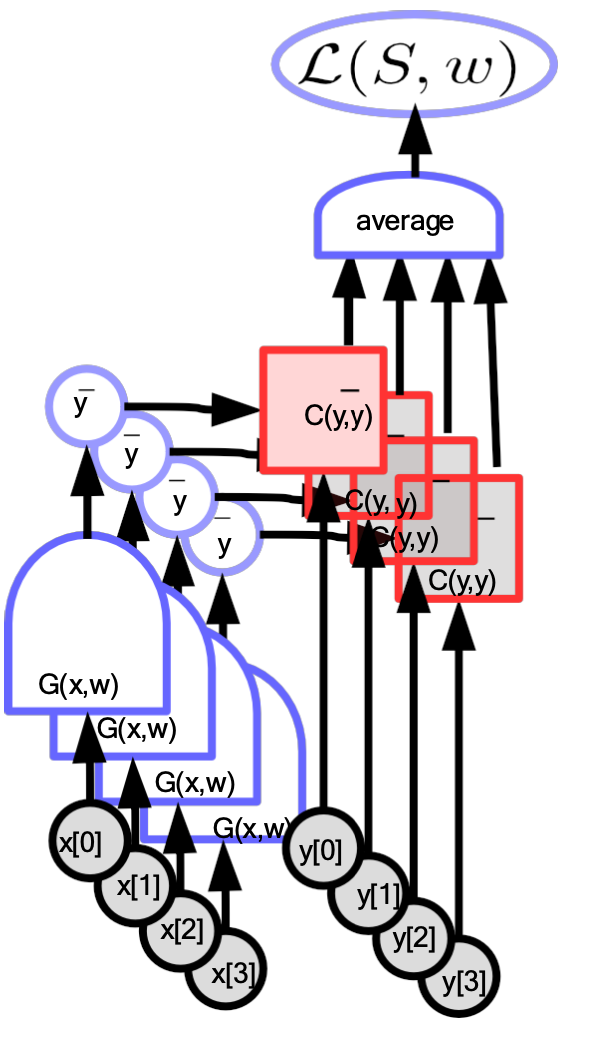
\includegraphics[width=0.30\linewidth]{figure/CostFunction.png}
    \caption{Rappresentazione tramite l'utilizzo di un grafico computazionale della funzione di costo, utilizzando la MSE}
    \label{fig:costFunction}
\end{figure}

\section{Reti Neurali}
Una Rete Neurale, tramite i nostri grafi computazionali, risulta essere una pila di blocchi funzionali lineari e non lineari. Le loro entità fondamentali prendono il nome di neuroni(Figura~\ref{fig:neuralNet}). Ogni \textbf{neurone} calcola una somma pesata degli input ricevuti e applica una funzione di attivazione per introdurre non linearità nel modello. Questa architettura, permette alla rete di apprendere rappresentazioni complesse dei dati. Un singolo neurone in una rete neurale può essere rappresentato come segue:
\begin{equation}
    z = \sum_{i=1}^{n} w_i x_i + b
\end{equation}
Dove $w_i$ sono i pesi associati agli input $x_i$, e relativi al bias $b$ (un peso costante che va sommato agli altri pesi). Successivamente, viene applicata una funzione di attivazione $\sigma(z)$ in modo tale da ottenere un output finale:
\begin{equation}
    y = \sigma(z)
\end{equation}

Le reti neurali, sono strutture complesse composte da tanti neuroni, i quali possono essere completamente collegati fra loro, generando le \textit{Fully-Connected Neural Network}, oppure collegate parzialemente creandone di diversa tipologia, i neuroni vengono concatenati formando diversi strati, dando la possibilità di formare delle archittetture profonde, composte da diversi strati.

\begin{figure}[ht]
    \centering
    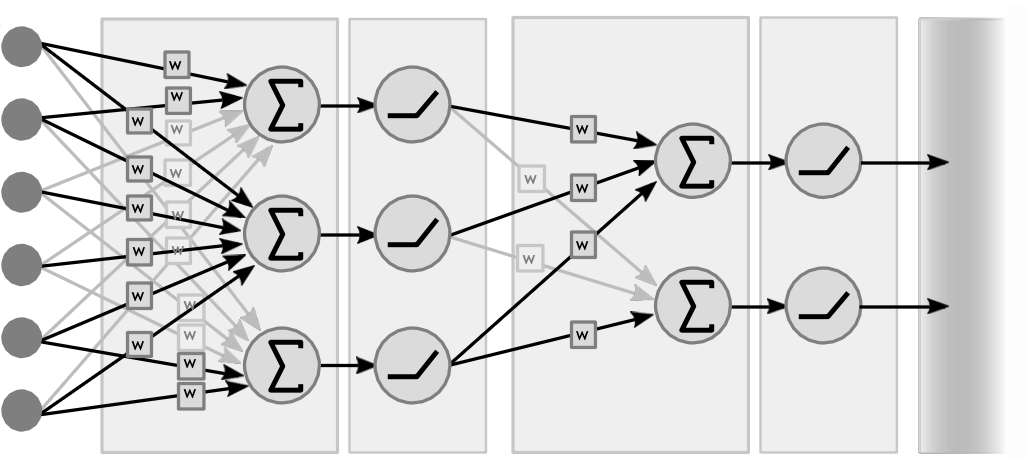
\includegraphics[width=0.85\textwidth]{figure/NeuralNet.png}
    \caption{Figura rappresentativa di un esempio di rete neurale con diversi strati nella sua architettura.}
    \label{fig:neuralNet}
\end{figure}

\section{Backpropagation}
La \textbf{Backpropagation} (retropropagazione), è uno degli algoritmi principali quando si parla di reti neurali, poiché permette di allenare la rete, basandosi sulla \textbf{discesa del gradiente}.
\begin{Definizione}
    La discesa del gradiente è un algoritmo di ottimizzazione che trova il valore minimo di una funzione, spostandosi iterativamente nella direzione opposta al suo gradiente. 
\end{Definizione}
L'idea della Backpropagation, è quella di propagare all'indietro l'errore generato dalla predizione e dal valore effettivo, in modo da aggiornare i pesi della rete, in modo che venga ridotto l'errore complessivo (la loss function). Il processo di Backpropagation consente di calcolare i gradienti dell'errore, rispetto ai pesi della rete e poter propagare questi gradienti attraverso la rete all'indietro, in modo tale da aggiornare i pesi e ottenere dei risultati sempre più accurati di volta in volta fintantoché non si raggiunge a una convergenza dei valori dei pesi.

\subsection{Calcolo dei Gradienti}
Il cuore della Backpropagation risiede nel calcolo dei gradienti della loss function rispetto ai pesi, utilizzando la \textbf{regola della catena}.
\begin{Definizione}
    La regola della catena afferma che se $f(x)$ e $g(x)$ sono funzioni derivabili, allora la derivata della funzione composta $h(x) = f(g(x))$ è:
    \[
    \frac{\partial h}{\partial x} = \frac{\partial f}{\partial g} \cdot \frac{\partial g}{\partial x}
    \]
\end{Definizione}
\marginpar{\href{https://cannydatascience.medium.com/backpropagation-come-apprende-una-rete-neurale-91c0c900fbc}{Approfondimento sulla Backpropagation}}
L'algoritmo di Backpropagation calcola i gradienti da ogni layer e li propaga all'indietro, aggiornando i pesi della rete. Il gradiente indica la direzione nella quale i pesi devono essere aggiornati per ridurre l'errore complessivo. La formula generale per la derivata della funzione di costo rispetto ai pesi è la seguente:
\begin{equation}
    \frac{\partial C}{\partial W} = \frac{\partial C}{\partial y} \cdot \frac{\partial y}{\partial W}
\end{equation}
Dove $C$ rappresenta la funzione di costo, $y$ l'output del modello e $W$ il peso da aggiornare. Questo processo viene ripetuto per ogni livello della rete, fino all'ottimizzazione del valore dei pesi. Questa procedura può essere facilmente sintetizzata in un grafo computazionale (Figura~\ref{fig:backPropGraph}). Nell'algoritmo della backpropagation è possibile applicare qualunque grafo che sia diretto e aciclico. Nel caso in cui il grafo presentasse dei loop, sarà necessario scioglierli.

\begin{figure}
    \centering
    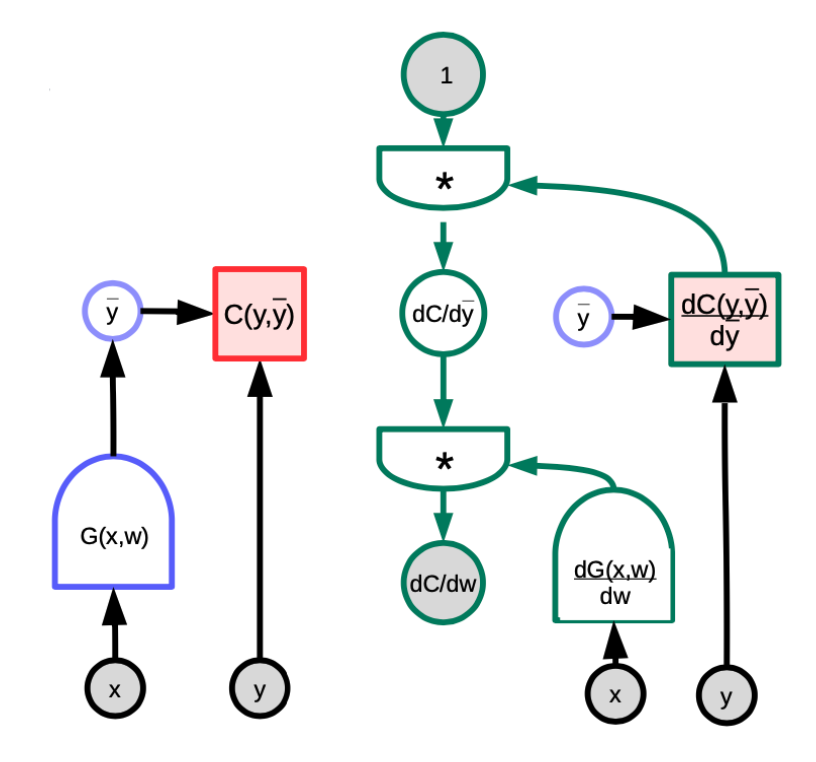
\includegraphics[width=0.5\linewidth]{figure/BackPropGraph.png}
    \caption{Grafo computazionale della Backpropagation, che si integra con quello già precedentemente visto della funzione di costo in modo tale da raffinare gli esiti finali correggendosi dinamicamente}
    \label{fig:backPropGraph}
\end{figure}

\section{Problemi della Backpropagation}
La Backpropagation soffre di due principali problemi ossia quello del \textit{gradiente che scompare} e quello che \textit{esplode}. Questi due problemi si verificano quando il gradiente della funzione di costo, rispetto ai pesi, risulta essere molto piccolo o molto grande nei livelli più profondi della rete.

\begin{itemize}
    \item \textbf{Gradiente che scompare:} nelle reti molto profonde, i gradienti calcolati per i livelli iniziali diventano sempre più piccoli man mano che vengono propagati all'indietro. Questo provoca degli aggiornamenti minimi dei pesi nei primi livelli, rallentando drasticamente l'addestramento o impedendo alla rete di apprendere;
    \item \textbf{Gradiente che esplode:} al contrario, se i gradienti aumentano esponenzialmente durante la propagazione all'indietro, i pesi della rete possono diventare estremamente grandi, portando a instabilità nell'addestramento e rendendone difficile la convergenza.
\end{itemize}

Con il passare degli anni il Machine Learning evolvendosi e specializzandosi nel Deep Learning, portando allo sviluppo di diverse soluzioni per queste problematiche:

\begin{enumerate}
    \item \textbf{Funzioni di attivazione avanzate:} L'utilizzo di altre funzioni come \textbf{ReLU} (Rectified Linear Unit) la quale ha ridotto il problema del gradiente che scompare rispetto alla funzione $\operatorname{sigmoid}$ e $\operatorname{tanh}$. Varianti come $\operatorname{Leaky\,ReLU}$ e $\operatorname{Parametric\,ReLU}$ migliorano ulteriormente l'apprendimento;
    \item \textbf{Inizializzazione dei pesi:} Metodi di inizializzazione dei pesi come \textbf{Xavier} per l'assegnamento dei pesi stabilizzano i gradienti all'inizio dell'addestramento;
    \item \textbf{Batch Normalization:} Tecnica la quale permette di normalizzare le attivazioni intermedie riducendo la varianza dei gradienti durante la propagazione.
\end{enumerate}

L'introduzione infatti di queste e altre tecniche, hanno permesso al Deep Learning di diventare un campo di studio sempre più interessante, divenendo anche più efficace come tecnica rispetto all'utilizzo di metodi tradizionali postulati dal Machine Learning.

\section{Implementazione con PyTorch}
Per effettuare una parallelizzazione della teoria, con l'aspetto implementativo del Deep Learning, quì mostriamo come implementare una rete neurale utilizzando \textbf{PyTorch}, per far ciò possiamo utilizzare la classe \texttt{nn.Module} in modo tale da definire la nostra architettura. Di seguito un esempio di una semplice rete con due livelli nascosti:
\\
\begin{python}[frame=trBL]
    import torch
    from torch import nn

    class MyNet(nn.Module):
        def __init__(self, input_dim, hidden_dim, output_dim):
            super().__init__()
            self.fc1 = nn.Linear(input_dim, hidden_dim)
            self.fc2 = nn.Linear(hidden_dim, output_dim)
    
        def forward(self, x):
            x = torch.relu(self.fc1(x))
            x = self.fc2(x)
            return x
    model = MyNet(784, 128, 10)
\end{python}
\vspace{0.5em}
La rete in questo codice prende in input delle immagini di 28x28 pixel (convertite in vettori di 784 elementi), le elabora utilizzando un livello nascosto con 128 neuroni e produce infine un output di 10 neuroni corrispondenti alle 10 classi del dataset MNIST.